\documentclass[tikz,border=10pt]{standalone}

\usepackage{amsmath}
\usepackage{tikz}
\usepackage{hyperref}
\usepackage{tkz-graph}
\usetikzlibrary{arrows}
\usetikzlibrary{petri}

\newcommand*{\rechterWinkel}[3]{% #1 = point, #2 = start angle, #3 = radius
   \draw[shift={(#2:#3)}] (#1) arc[start angle=#2, delta angle=90, radius = #3];
   \fill[shift={(#2+45:#3/2)}] (#1) circle[radius=1.25\pgflinewidth];
}

\begin{document}
	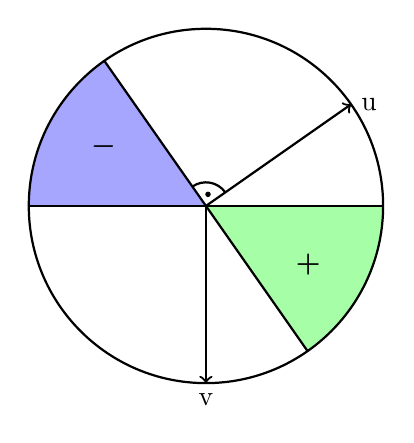
\begin{tikzpicture}[
		-,
		auto,
		node distance=1.6cm,
		thick
	]
	  	\tikzstyle{neuron}=[
	  		circle,
	  		draw,
	  		minimum size=17pt,
	  		inner sep=0pt
	  	]
	  	
	  	\fill[fill=green!35] (0,0) -- (-55:2.25cm) arc (-55:0:2.25cm) -- cycle;
	  	\fill[fill=blue!35] (0,0) -- (125:2.25cm) arc (125:180:2.25cm) -- cycle;
	  	\draw (0,0) circle (2.25cm);
%	  	\draw[->] (-3,0) -- (3,0) node[right] {x};		
%	  	\draw[->] (0,-3) -- (0,3) node[right] {y};	
	  	\draw[->] (0,0) -- (35:2.25cm) node[right] {u};
	  	\draw[->] (0,0) -- (-90:2.25cm) node[below] {v};
	  	\draw (180:2.25cm) -- (0:2.25cm);
	  	\draw (125:2.25cm) -- (-55:2.25cm);
	  	\rechterWinkel{0,0}{35}{0.3}; 
	  	\node at (1.3,-0.75) {$\boldsymbol{+}$};
	  	\node at (-1.3,0.75) {$\boldsymbol{-}$};
	\end{tikzpicture}
\end{document}